\documentclass[twoside]{book}

% Packages required by doxygen
\usepackage{fixltx2e}
\usepackage{calc}
\usepackage{doxygen}
\usepackage{graphicx}
\usepackage[utf8]{inputenc}
\usepackage{makeidx}
\usepackage{multicol}
\usepackage{multirow}
\PassOptionsToPackage{warn}{textcomp}
\usepackage{textcomp}
\usepackage[nointegrals]{wasysym}
\usepackage[table]{xcolor}

% Font selection
\usepackage[T1]{fontenc}
\usepackage{mathptmx}
\usepackage[scaled=.90]{helvet}
\usepackage{courier}
\usepackage{amssymb}
\usepackage{sectsty}
\renewcommand{\familydefault}{\sfdefault}
\allsectionsfont{%
  \fontseries{bc}\selectfont%
  \color{darkgray}%
}
\renewcommand{\DoxyLabelFont}{%
  \fontseries{bc}\selectfont%
  \color{darkgray}%
}
\newcommand{\+}{\discretionary{\mbox{\scriptsize$\hookleftarrow$}}{}{}}

% Page & text layout
\usepackage{geometry}
\geometry{%
  a4paper,%
  top=2.5cm,%
  bottom=2.5cm,%
  left=2.5cm,%
  right=2.5cm%
}
\tolerance=750
\hfuzz=15pt
\hbadness=750
\setlength{\emergencystretch}{15pt}
\setlength{\parindent}{0cm}
\setlength{\parskip}{0.2cm}
\makeatletter
\renewcommand{\paragraph}{%
  \@startsection{paragraph}{4}{0ex}{-1.0ex}{1.0ex}{%
    \normalfont\normalsize\bfseries\SS@parafont%
  }%
}
\renewcommand{\subparagraph}{%
  \@startsection{subparagraph}{5}{0ex}{-1.0ex}{1.0ex}{%
    \normalfont\normalsize\bfseries\SS@subparafont%
  }%
}
\makeatother

% Headers & footers
\usepackage{fancyhdr}
\pagestyle{fancyplain}
\fancyhead[LE]{\fancyplain{}{\bfseries\thepage}}
\fancyhead[CE]{\fancyplain{}{}}
\fancyhead[RE]{\fancyplain{}{\bfseries\leftmark}}
\fancyhead[LO]{\fancyplain{}{\bfseries\rightmark}}
\fancyhead[CO]{\fancyplain{}{}}
\fancyhead[RO]{\fancyplain{}{\bfseries\thepage}}
\fancyfoot[LE]{\fancyplain{}{}}
\fancyfoot[CE]{\fancyplain{}{}}
\fancyfoot[RE]{\fancyplain{}{\bfseries\scriptsize Generated on Sun Mar 19 2017 00\+:38\+:27 for V\+R Robot Control by Doxygen }}
\fancyfoot[LO]{\fancyplain{}{\bfseries\scriptsize Generated on Sun Mar 19 2017 00\+:38\+:27 for V\+R Robot Control by Doxygen }}
\fancyfoot[CO]{\fancyplain{}{}}
\fancyfoot[RO]{\fancyplain{}{}}
\renewcommand{\footrulewidth}{0.4pt}
\renewcommand{\chaptermark}[1]{%
  \markboth{#1}{}%
}
\renewcommand{\sectionmark}[1]{%
  \markright{\thesection\ #1}%
}

% Indices & bibliography
\usepackage{natbib}
\usepackage[titles]{tocloft}
\setcounter{tocdepth}{3}
\setcounter{secnumdepth}{5}
\makeindex

% Hyperlinks (required, but should be loaded last)
\usepackage{ifpdf}
\ifpdf
  \usepackage[pdftex,pagebackref=true]{hyperref}
\else
  \usepackage[ps2pdf,pagebackref=true]{hyperref}
\fi
\hypersetup{%
  colorlinks=true,%
  linkcolor=blue,%
  citecolor=blue,%
  unicode%
}

% Custom commands
\newcommand{\clearemptydoublepage}{%
  \newpage{\pagestyle{empty}\cleardoublepage}%
}


%===== C O N T E N T S =====

\begin{document}

% Titlepage & ToC
\hypersetup{pageanchor=false,
             bookmarks=true,
             bookmarksnumbered=true,
             pdfencoding=unicode
            }
\pagenumbering{roman}
\begin{titlepage}
\vspace*{7cm}
\begin{center}%
{\Large V\+R Robot Control }\\
\vspace*{1cm}
{\large Generated by Doxygen 1.8.8}\\
\vspace*{0.5cm}
{\small Sun Mar 19 2017 00:38:27}\\
\end{center}
\end{titlepage}
\clearemptydoublepage
\tableofcontents
\clearemptydoublepage
\pagenumbering{arabic}
\hypersetup{pageanchor=true}

%--- Begin generated contents ---
\chapter{Main Page}
\label{index}\hypertarget{index}{}V\+R\+Control of Rapiro Robot using Node\+J\+S, Leap etc.\+fil 



\subsection*{Connecting to Rapiro-\/\+Pi via V\+N\+C}


\begin{DoxyEnumerate}
\item Download V\+N\+C Viewer from \href{https://www.realvnc.com/download/viewer/}{\tt https\+://www.\+realvnc.\+com/download/viewer/}
\item Click File -\/$>$ New Connection
\item Set V\+N\+C Server to {\ttfamily rapiro-\/pi.\+ddns.\+net\+:5900}
\item Set Name to {\ttfamily rapiro-\/pi-\/admin}
\item Click O\+K then double click on the newly created connection
\item Set Username to {\ttfamily admin}
\item Set Password to {\ttfamily V\+Rcontrol17}
\item Tick remember password
\item Click O\+K
\end{DoxyEnumerate}

\subsection*{Connecting to Rapiro-\/\+Pi via S\+S\+H}


\begin{DoxyEnumerate}
\item Open your preferred S\+S\+H Client Putty etc.
\item Set host to {\ttfamily rapiro-\/pi.\+ddns.\+net}
\item Set Port to {\ttfamily 22}
\item Username is {\ttfamily admin}
\item Password is {\ttfamily V\+Rcontrol17}
\end{DoxyEnumerate}

\subsection*{Connecting to Rapiro-\/\+Pi via F\+T\+P (Filezilla)}


\begin{DoxyEnumerate}
\item Download Filezilla from \href{https://filezilla-project.org/download.php?type=client}{\tt https\+://filezilla-\/project.\+org/download.\+php?type=client}
\item Click File -\/$>$ Site Manager
\item Click New Site and name {\ttfamily rapiro-\/pi-\/admin}
\item Set host to {\ttfamily rapiro-\/pi.\+ddns.\+net}
\item Set Port to {\ttfamily 22}
\item Set Protocol to {\ttfamily S\+F\+T\+P -\/ S\+S\+H File Transfer Protocol}
\item Set Logon Type to {\ttfamily Normal}
\item Set User to {\ttfamily admin}
\item Set Password to {\ttfamily V\+Rcontrol17}
\item Click connect
\end{DoxyEnumerate}

The connection will be saved and can be accessed again from Open Site Manager tab

\subsection*{Accessing Visual Studio Code in Rapiro-\/\+Pi}

Check to see if an instance is already open by hitting alt + tab or check the taskbar at the top (known bug sometimes disappears so use alt + tab or equivalent to O\+S you are on)


\begin{DoxyEnumerate}
\item If an instance is not running open the terminal
\item Type {\ttfamily cd vscode} then hit enter
\item Type {\ttfamily ./scripts/code.sh} then hit enter (be patient takes a while to fully load U\+I)
\end{DoxyEnumerate}

N\+O\+T\+E\+: The terminal command {\ttfamily ./scripts/code.sh} is what runs V\+S code so if you need to make any commands in terminal open a new terminal instance. Be careful not to accidentally close the terminal running V\+S code or data could be lost (V\+S code autosave feature is turned on but it is not a guarantee to prevent data loss) 
\chapter{input\+\_\+opencv filter plugin\+: cvfilter\+\_\+cpp}
\label{md_raspi-server_mjpg-streamer_plugins_input_opencv_filters_cvfilter_cpp_README}
\hypertarget{md_raspi-server_mjpg-streamer_plugins_input_opencv_filters_cvfilter_cpp_README}{}
This is just a demonstration plugin that shows how to create a bare minimum filter plugin for use with the mjpg-\/streamer input\+\_\+opencv plugin.

To create your own filter plugin, just copy filter\+\_\+cpp.\+cpp to your own project, and compile/link it with the same build of Open\+C\+V that mjpg-\/streamer is linked to.

C\+Make\+Lists.\+txt is specific to the mjpg-\/streamer build tree, and won't be useful outside of it. 
\chapter{input\+\_\+opencv filter plugin\+: cvfilter\+\_\+py}
\label{md_raspi-server_mjpg-streamer_plugins_input_opencv_filters_cvfilter_py_README}
\hypertarget{md_raspi-server_mjpg-streamer_plugins_input_opencv_filters_cvfilter_py_README}{}
This plugin allows you to use a Python 3.\+x script to process images received by mjpg-\/streamer. This has been tested with Python 3.\+4.

To run a Python 3.\+x script, you can do the following\+: \begin{DoxyVerb}mjpg_streamer -i "input_opencv.so --filter cvfilter_py.so --fargs path/to/filter.py"
\end{DoxyVerb}


\subsection*{Filter script }

Your script M\+U\+S\+T define a function called 'init\+\_\+filter', that takes zero arguments and returns a single callable. This returned callable must take a single argument (a numpy array), and returns a single object (a numpy array). A simple example follows\+:

```

def filter\+\_\+fn(img)\+: ''' \+:param img\+: A numpy array representing the input image \+:returns\+: A numpy array to send to the mjpg-\/streamer output plugin ''' return img

def init\+\_\+filter()\+: return filter\+\_\+fn

```

For a more complex example, see the included example\+\_\+filter.\+py

\subsection*{Known Issues }

When mjpg-\/streamer is terminated, a {\ttfamily Key\+Error} is raised in the threading module. While annoying, it's harmless. Most likely it happens because the python interpreter is destroyed on the wrong thread.

\subsection*{T\+O\+D\+O }

After going through all of this effort to create the code for this module, I bet it can be done a lot simpler via cython.

\subsection*{Authors }

Dustin Spicuzza (\href{mailto:dustin@virtualroadside.com}{\tt dustin@virtualroadside.\+com}) 
\chapter{mjpg-\/streamer input plugin\+: input\+\_\+opencv}
\label{md_raspi-server_mjpg-streamer_plugins_input_opencv_README}
\hypertarget{md_raspi-server_mjpg-streamer_plugins_input_opencv_README}{}
This input plugin uses Open\+C\+V to read from supported video sources, optionally running the image through a filter plugin that can be specified on the command line.

If you're not using the image filtering functionality of this plugin, you're probably better off using some other input plugin as this plugin will probably consume more C\+P\+U resources.

This plugin has only been tested with Open\+C\+V 3.\+1.\+0, will probably not work with Open\+C\+V 2.\+x without some adjustments.

\section*{Usage }

\subsection*{``` }

\subsection*{Help for input plugin..\+: Open\+C\+V Input plugin }

The following parameters can be passed to this plugin\+:

\mbox{[}-\/d $\vert$ --device \mbox{]}.......\+: video device to open (your camera) \mbox{[}-\/r $\vert$ --resolution \mbox{]}...\+: the resolution of the video device, can be one of the following strings\+: Q\+Q\+V\+G\+A Q\+C\+I\+F C\+G\+A Q\+V\+G\+A C\+I\+F V\+G\+A S\+V\+G\+A X\+G\+A H\+D S\+X\+G\+A U\+X\+G\+A F\+H\+D

or a custom value like the following example\+: 640x480 \mbox{[}-\/f $\vert$ --fps \mbox{]}..........\+: frames per second \subsection*{\mbox{[}-\/q $\vert$ --quality \mbox{]} .....\+: set quality of J\+P\+E\+G encoding }

Optional parameters (may not be supported by all cameras)\+:

\mbox{[}-\/br \mbox{]}.................\+: Set image brightness (integer) \mbox{[}-\/co \mbox{]}.................\+: Set image contrast (integer) \mbox{[}-\/sh \mbox{]}.................\+: Set image sharpness (integer) \mbox{[}-\/sa \mbox{]}.................\+: Set image saturation (integer) \mbox{[}-\/ex \mbox{]}.................\+: Set exposure (off, or integer) \subsection*{\mbox{[}-\/gain \mbox{]}...............\+: Set gain (integer) }

Optional filter plugin\+: \mbox{[} -\/filter \mbox{]}............\+: filter plugin .so \subsection*{\mbox{[} -\/fargs \mbox{]}.............\+: filter plugin arguments }

```

\section*{Filter plugins }

You can specify a filter plugin to load via the \char`\"{}-\/-\/filter\char`\"{} argument\+: \begin{DoxyVerb}mjpg_streamer -i "input_opencv.so --filter cvfilter_cpp.so" .. 
\end{DoxyVerb}


The following plugins are included\+:


\begin{DoxyItemize}
\item cvfilter\+\_\+cpp\+: barebones example
\item cvfilter\+\_\+py\+: Embeds a python interpreter to allow you to create a filter script in Python
\end{DoxyItemize}

\subsection*{Authors }

Dustin Spicuzza (\href{mailto:dustin@virtualroadside.com}{\tt dustin@virtualroadside.\+com}) 
\chapter{mjpg-\/streamer input plugin\+: input\+\_\+raspicam}
\label{md_raspi-server_mjpg-streamer_plugins_input_raspicam_README}
\hypertarget{md_raspi-server_mjpg-streamer_plugins_input_raspicam_README}{}
M\+J\+P\+E\+G Streamer with raspicam input plugin (based on raspistill mmal source code)

\section*{Discussion / Questions / Help }

Probably best in this thread \href{http://www.raspberrypi.org/phpBB3/viewtopic.php?f=43&t=45178}{\tt http\+://www.\+raspberrypi.\+org/php\+B\+B3/viewtopic.\+php?f=43\&t=45178}

\section*{Instructions }

If you ran the basic build, you can run from the mjpeg streamer experimental folder with\+: ``` export L\+D\+\_\+\+L\+I\+B\+R\+A\+R\+Y\+\_\+\+P\+A\+T\+H=. ./mjpg\+\_\+streamer -\/o \char`\"{}output\+\_\+http.\+so -\/w ./www\char`\"{} -\/i \char`\"{}input\+\_\+raspicam.\+so\char`\"{} ```

You can specify options, like in raspivid\+: ``` export L\+D\+\_\+\+L\+I\+B\+R\+A\+R\+Y\+\_\+\+P\+A\+T\+H=. ./mjpg\+\_\+streamer -\/o \char`\"{}output\+\_\+http.\+so -\/w ./www\char`\"{} -\/i \char`\"{}input\+\_\+raspicam.\+so -\/x 1280 -\/y 720 -\/fps 15 -\/ex night\char`\"{} ```

It does support upto 1080p 30fps, but the bandwidth produced would be more than the usb bus (and therefore ethernet port / wifi dongle) can provide. 720p 15fps is a good compromise.

Here's some help for this input plugin\+: \subsection*{``` }

\subsection*{Help for input plugin..\+: raspicam input plugin }

The following parameters can be passed to this plugin\+:

\mbox{[}-\/fps $\vert$ --framerate\mbox{]}...\+: set video framerate, default 5 frame/sec \mbox{[}-\/x $\vert$ --width \mbox{]}........\+: width of frame capture, default 640 \mbox{[}-\/y $\vert$ --height\mbox{]}........\+: height of frame capture, default 480 \mbox{[}-\/quality\mbox{]}.............\+: set J\+P\+E\+G quality 0-\/100, default 85 \mbox{[}-\/usestills\mbox{]}...........\+: uses stills mode instead of video mode \mbox{[}-\/preview\mbox{]}.............\+: enable full screen preview

-\/sh \+: Set image sharpness (-\/100 to 100) -\/co \+: Set image contrast (-\/100 to 100) -\/br \+: Set image brightness (0 to 100) -\/sa \+: Set image saturation (-\/100 to 100) -\/\+I\+S\+O \+: Set capture I\+S\+O -\/vs \+: Turn on video stabilisation -\/ev \+: Set E\+V compensation -\/ex \+: Set exposure mode (see raspistill notes) -\/awb \+: Set A\+W\+B mode (see raspistill notes) -\/ifx \+: Set image effect (see raspistill notes) -\/cfx \+: Set colour effect (U\+:V) -\/mm \+: Set metering mode (see raspistill notes) -\/rot \+: Set image rotation (0-\/359) -\/stats \+: Compute image stats for each picture (reduces noise) -\/drc \+: Dynamic range compensation level (see raspistill notes) -\/hf \+: Set horizontal flip \subsection*{-\/vf \+: Set vertical flip }

``` Some of the camera options like I\+S\+O may not work due to it not working in the mmal-\/libs.

Video mode is the default as it allows much smoother video (higher framerates). Stills mode allows you to use the full-\/frame of the sensor, but has a max framerate of around 8fps, probably less. Use stills mode with low F\+P\+S (e.\+g. 1 or 2).

In order to have preview output shown on the raspi screen add the -\/preview option.

This should run indefinitely. ctrl-\/c closes mjpeg streamer and raspicam gracefully.

Based on \href{https://github.com/raspberrypi/userland/blob/master/host_applications/linux/apps/raspicam/RaspiStill.c}{\tt https\+://github.\+com/raspberrypi/userland/blob/master/host\+\_\+applications/linux/apps/raspicam/\+Raspi\+Still.\+c} modified mmal header and source files from \href{https://github.com/raspberrypi/userland/tree/master/interface/mmal}{\tt https\+://github.\+com/raspberrypi/userland/tree/master/interface/mmal} 
\chapter{mjpg-\/streamer input plugin\+: input\+\_\+uvc}
\label{md_raspi-server_mjpg-streamer_plugins_input_uvc_README}
\hypertarget{md_raspi-server_mjpg-streamer_plugins_input_uvc_README}{}
This plugin provides J\+P\+E\+G data from V4\+L/\+V4\+L2 compatible webcams.

\section*{Usage }

\begin{DoxyVerb}mjpg_streamer -i 'input_uvc.so [options]'
\end{DoxyVerb}


\subsection*{``` }

\subsection*{Help for input plugin..\+: U\+V\+C webcam grabber }

The following parameters can be passed to this plugin\+:

\mbox{[}-\/d $\vert$ --device \mbox{]}.......\+: video device to open (your camera) \mbox{[}-\/r $\vert$ --resolution \mbox{]}...\+: the resolution of the video device, can be one of the following strings\+: Q\+S\+I\+F Q\+C\+I\+F C\+G\+A Q\+V\+G\+A C\+I\+F V\+G\+A S\+V\+G\+A X\+G\+A S\+X\+G\+A or a custom value like the following example\+: 640x480 \mbox{[}-\/f $\vert$ --fps \mbox{]}..........\+: frames per second (activates Y\+U\+Y\+V format, disables M\+J\+P\+E\+G) \mbox{[}-\/m $\vert$ --minimum\+\_\+size \mbox{]}.\+: drop frames smaller then this limit, useful if the webcam produces small-\/sized garbage frames may happen under low light conditions \mbox{[}-\/e $\vert$ --every\+\_\+frame \mbox{]}..\+: drop all frames except numbered \mbox{[}-\/n $\vert$ --no\+\_\+dynctrl \mbox{]}...\+: do not initalize dynctrls of Linux-\/\+U\+V\+C driver \mbox{[}-\/l $\vert$ --led \mbox{]}..........\+: switch the L\+E\+D \char`\"{}on\char`\"{}, \char`\"{}off\char`\"{}, let it \char`\"{}blink\char`\"{} or leave \subsection*{it up to the driver using the value \char`\"{}auto\char`\"{} }

\subsection*{\mbox{[}-\/t $\vert$ --tvnorm \mbox{]} ......\+: set T\+V-\/\+Norm pal, ntsc or secam }

Optional parameters (may not be supported by all cameras)\+:

\mbox{[}-\/br \mbox{]}.................\+: Set image brightness (auto or integer) \mbox{[}-\/co \mbox{]}.................\+: Set image contrast (integer) \mbox{[}-\/sh \mbox{]}.................\+: Set image sharpness (integer) \mbox{[}-\/sa \mbox{]}.................\+: Set image saturation (integer) \mbox{[}-\/cb \mbox{]}.................\+: Set color balance (auto or integer) \mbox{[}-\/wb \mbox{]}.................\+: Set white balance (auto or integer) \mbox{[}-\/ex \mbox{]}.................\+: Set exposure (auto, shutter-\/priority, aperature-\/priority, or integer) \mbox{[}-\/bk \mbox{]}.................\+: Set backlight compensation (integer) \mbox{[}-\/rot \mbox{]}................\+: Set image rotation (0-\/359) \mbox{[}-\/hf \mbox{]}.................\+: Set horizontal flip (true/false) \mbox{[}-\/vf \mbox{]}.................\+: Set vertical flip (true/false) \mbox{[}-\/pl \mbox{]}.................\+: Set power line filter (disabled, 50hz, 60hz, auto) \mbox{[}-\/gain \mbox{]}...............\+: Set gain (auto or integer) \subsection*{\mbox{[}-\/cagc \mbox{]}...............\+: Set chroma gain control (auto or integer) }

``` 
\chapter{mjpg-\/streamer output plugin\+: output\+\_\+http}
\label{md_raspi-server_mjpg-streamer_plugins_output_http_README}
\hypertarget{md_raspi-server_mjpg-streamer_plugins_output_http_README}{}
This plugin streams J\+P\+E\+G data from input plugins via H\+T\+T\+P.

\section*{Usage }

\begin{DoxyVerb}mjpg_streamer [input plugin options] -o 'output_http.so [options]'
\end{DoxyVerb}


\subsection*{``` }

The following parameters can be passed to this plugin\+:

\mbox{[}-\/w $\vert$ --www \mbox{]}...........\+: folder that contains webpages in flat hierarchy (no subfolders) \mbox{[}-\/p $\vert$ --port \mbox{]}..........\+: T\+C\+P port for this H\+T\+T\+P server \mbox{[}-\/c $\vert$ --credentials \mbox{]}...\+: ask for \char`\"{}username\+:password\char`\"{} on connect \subsection*{\mbox{[}-\/n $\vert$ --nocommands \mbox{]}....\+: disable execution of commands }

```

\subsection*{Browser/\+V\+L\+C }

To view the stream use V\+L\+C or Firefox/\+Chrome and open the U\+R\+L\+: \begin{DoxyVerb}http://127.0.0.1:8080/?action=stream
\end{DoxyVerb}


If there are multiple input plugins, you can access each stream individually\+: \begin{DoxyVerb}http://127.0.0.1:8080/?action=stream_0
http://127.0.0.1:8080/?action=stream_1
\end{DoxyVerb}


To do the same as the G\+E\+T request above using N\+S\+U\+R\+L\+Session in Objective-\/\+C, a P\+O\+S\+T request seems to work\+: \begin{DoxyVerb}POST http://127.0.0.1:8080/stream 
\end{DoxyVerb}


To view a single J\+P\+E\+G just open this U\+R\+L\+: \begin{DoxyVerb}http://127.0.0.1:8080/?action=snapshot
\end{DoxyVerb}


\subsection*{mplayer }

To play the H\+T\+T\+P M-\/\+J\+P\+E\+G stream with mplayer\+: \begin{DoxyVerb}# mplayer -fps 30 -demuxer lavf "http://127.0.0.1:8080/?action=stream&ignored.mjpg"
\end{DoxyVerb}


It might be necessary to configure mplayer to prefer I\+Pv4 instead of I\+Pv6\+: \begin{DoxyVerb}# vi ~./mplayer/config
add or change the option: prefer-ipv4=yes
\end{DoxyVerb}


\section*{Notes }

If you would like to replace a Webcam\+X\+P based system with an mjpg-\/streamer based you may use the W\+X\+P\+\_\+\+C\+O\+M\+P\+A\+T argument to cmake. If you compile with this argument the mjpg stream will be available as cam\+\_\+1.\+mjpg and the still jpg snapshot as cam\+\_\+1.\+jpg. \begin{DoxyVerb}# mkdir _build
# cd _build && cmake -DWXP_COMPAT=ON ..
# make\end{DoxyVerb}
 
\chapter{mjpg-\/streamer output plugin\+: output\+\_\+viewer}
\label{md_raspi-server_mjpg-streamer_plugins_output_viewer_README}
\hypertarget{md_raspi-server_mjpg-streamer_plugins_output_viewer_README}{}
This is a simple plugin that will display the input plugin stream in an S\+D\+L window.

You must have libsdl-\/devel installed (or similar) in order for this plugin to be compiled \& installed.

\section*{Usage }

\begin{DoxyVerb}mjpg_streamer [input plugin options] -o 'output_viewer.so' \end{DoxyVerb}
 
\chapter{mjpg-\/streamer}
\label{md_raspi-server_mjpg-streamer_README}
\hypertarget{md_raspi-server_mjpg-streamer_README}{}
Currently no issues are known, but since this software is quite young and not used widely it may cause problems. You must really know what you are doing, if you use this software. If you want to use the software you are obliged to check if the sourcecode does what you expect it to do and take the risk yourself to use it.

\section*{Usage }

When launching mjpg-\/streamer, you specify one or more input plugins and an output plugin. For example, to stream a V4\+L compatible webcam via an H\+T\+T\+P server (the most common use case), you can do something like this\+: \begin{DoxyVerb}mjpg_streamer -i input_uvc.so -o output_http.so
\end{DoxyVerb}


Each plugin supports various options, you can view the plugin's options via its {\ttfamily -\/-\/help} option\+: \begin{DoxyVerb}mjpg_streamer -i 'input_uvc.so --help'
\end{DoxyVerb}


More examples can be found in the start.\+sh bash script.

\section*{Plugin documentation }

Input plugins\+:


\begin{DoxyItemize}
\item input\+\_\+file
\item input\+\_\+http
\item input\+\_\+opencv (documentation)
\item input\+\_\+ptp2
\item input\+\_\+raspicam (documentation)
\item input\+\_\+uvc (documentation)
\end{DoxyItemize}

Output plugins\+:


\begin{DoxyItemize}
\item output\+\_\+file
\item output\+\_\+http (documentation)
\item output\+\_\+rtsp
\item output\+\_\+udp
\item output\+\_\+viewer (documentation) 
\end{DoxyItemize}
\chapter{Class Index}
\section{Class List}
Here are the classes, structs, unions and interfaces with brief descriptions\+:\begin{DoxyCompactList}
\item\contentsline{section}{\hyperlink{classnewRobot}{new\+Robot} \\*Class for holding our robot structure for cylon. Includes the connection, device \& work function }{\pageref{classnewRobot}}{}
\item\contentsline{section}{\hyperlink{classserver}{server} \\*Server objcet started on port 8001 }{\pageref{classserver}}{}
\end{DoxyCompactList}

\chapter{File Index}
\section{File List}
Here is a list of all documented files with brief descriptions\+:\begin{DoxyCompactList}
\item\contentsline{section}{arduino-\/sketch/\hyperlink{arduino-sketch_8ino}{arduino-\/sketch.\+ino} \\*Arduino motor controller for Zumo\+Motors }{\pageref{arduino-sketch_8ino}}{}
\item\contentsline{section}{leap-\/client/\hyperlink{client_8js}{client.\+js} \\*Node client for parsing hand gestures from L\+E\+A\+P motion }{\pageref{client_8js}}{}
\item\contentsline{section}{raspi-\/server/\hyperlink{server_8js}{server.\+js} \\*Main code for our Node\+J\+S Raspberry P\+I server }{\pageref{server_8js}}{}
\item\contentsline{section}{raspi-\/server/business/\hyperlink{raspiBusiness_8js}{raspi\+Business.\+js} \\*Module for parsing Zumo movement commands received via H\+T\+T\+P requests }{\pageref{raspiBusiness_8js}}{}
\item\contentsline{section}{raspi-\/server/business/\hyperlink{zumoInterface_8js}{zumo\+Interface.\+js} \\*Zumo Node\+J\+S interface }{\pageref{zumoInterface_8js}}{}
\end{DoxyCompactList}

\chapter{Class Documentation}
\hypertarget{classnewRobot}{\section{new\+Robot Class Reference}
\label{classnewRobot}\index{new\+Robot@{new\+Robot}}
}


Class for holding our robot structure for cylon. Includes the connection, device \& work function.  




\subsection{Detailed Description}
Class for holding our robot structure for cylon. Includes the connection, device \& work function. 

The documentation for this class was generated from the following file\+:\begin{DoxyCompactItemize}
\item 
leap-\/client/\hyperlink{client_8js}{client.\+js}\end{DoxyCompactItemize}

\hypertarget{classserver}{\section{server Class Reference}
\label{classserver}\index{server@{server}}
}


Server objcet started on port 8001.  




\subsection{Detailed Description}
Server objcet started on port 8001. 

The documentation for this class was generated from the following file\+:\begin{DoxyCompactItemize}
\item 
raspi-\/server/\hyperlink{server_8js}{server.\+js}\end{DoxyCompactItemize}

\chapter{File Documentation}
\hypertarget{arduino-sketch_8ino}{\section{arduino-\/sketch/arduino-\/sketch.ino File Reference}
\label{arduino-sketch_8ino}\index{arduino-\/sketch/arduino-\/sketch.\+ino@{arduino-\/sketch/arduino-\/sketch.\+ino}}
}


Arduino motor controller for Zumo\+Motors.  


{\ttfamily \#include $<$Zumo\+Motors.\+h$>$}\\*
Include dependency graph for arduino-\/sketch.ino\+:\nopagebreak
\begin{figure}[H]
\begin{center}
\leavevmode
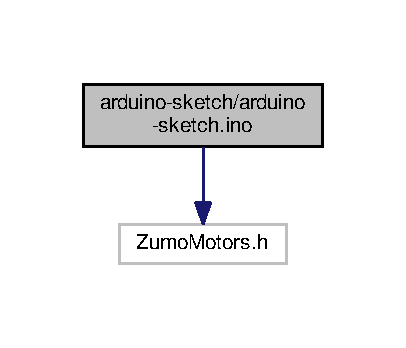
\includegraphics[width=195pt]{arduino-sketch_8ino__incl}
\end{center}
\end{figure}
\subsection*{Macros}
\begin{DoxyCompactItemize}
\item 
\hypertarget{arduino-sketch_8ino_a764dbd349d8621accd792ee5210a3f74}{\#define {\bfseries C\+H\+A\+R\+\_\+\+F\+O\+R\+W\+A\+R\+D}~'W'}\label{arduino-sketch_8ino_a764dbd349d8621accd792ee5210a3f74}

\item 
\hypertarget{arduino-sketch_8ino_a1681b01a2698687a9b6aedd45b796f40}{\#define {\bfseries C\+H\+A\+R\+\_\+\+B\+A\+C\+K\+W\+A\+R\+D}~'S'}\label{arduino-sketch_8ino_a1681b01a2698687a9b6aedd45b796f40}

\item 
\hypertarget{arduino-sketch_8ino_aa05ecc497d01a93be5dd62ddaee54a75}{\#define {\bfseries C\+H\+A\+R\+\_\+\+L\+E\+F\+T}~'A'}\label{arduino-sketch_8ino_aa05ecc497d01a93be5dd62ddaee54a75}

\item 
\hypertarget{arduino-sketch_8ino_a94f7d75840f1acbd2c2acd01fc115d88}{\#define {\bfseries C\+H\+A\+R\+\_\+\+R\+I\+G\+H\+T}~'D'}\label{arduino-sketch_8ino_a94f7d75840f1acbd2c2acd01fc115d88}

\item 
\hypertarget{arduino-sketch_8ino_a245db460299318b2a2b61c2f884c1d19}{\#define {\bfseries C\+H\+A\+R\+\_\+\+S\+T\+O\+P}~'Q'}\label{arduino-sketch_8ino_a245db460299318b2a2b61c2f884c1d19}

\item 
\hypertarget{arduino-sketch_8ino_ae84e9944a7983ebfabc5ad16c9fbc04d}{\#define {\bfseries N\+O\+\_\+\+S\+P\+E\+E\+D}~0}\label{arduino-sketch_8ino_ae84e9944a7983ebfabc5ad16c9fbc04d}

\item 
\hypertarget{arduino-sketch_8ino_ac2cd96d53dd3ba6407db6766c3d92b26}{\#define {\bfseries M\+A\+X\+\_\+\+S\+P\+E\+E\+D}~200}\label{arduino-sketch_8ino_ac2cd96d53dd3ba6407db6766c3d92b26}

\item 
\hypertarget{arduino-sketch_8ino_afa9188776d909e94ead6cf6ffbbdd1e8}{\#define {\bfseries T\+U\+R\+N\+\_\+\+S\+P\+E\+E\+D}~185}\label{arduino-sketch_8ino_afa9188776d909e94ead6cf6ffbbdd1e8}

\end{DoxyCompactItemize}
\subsection*{Functions}
\begin{DoxyCompactItemize}
\item 
void \hyperlink{arduino-sketch_8ino_a4fc01d736fe50cf5b977f755b675f11d}{setup} ()
\begin{DoxyCompactList}\small\item\em Runs once at boot of arduino. \end{DoxyCompactList}\item 
void \hyperlink{arduino-sketch_8ino_afe461d27b9c48d5921c00d521181f12f}{loop} ()
\begin{DoxyCompactList}\small\item\em System loop that is ran continuously. \end{DoxyCompactList}\end{DoxyCompactItemize}
\subsection*{Variables}
\begin{DoxyCompactItemize}
\item 
\hypertarget{arduino-sketch_8ino_a107e8fa5802407f91589286783cb7c5d}{Zumo\+Motors {\bfseries motors}}\label{arduino-sketch_8ino_a107e8fa5802407f91589286783cb7c5d}

\end{DoxyCompactItemize}


\subsection{Detailed Description}
Arduino motor controller for Zumo\+Motors. 

\begin{DoxyAuthor}{Author}
Jack Allister -\/ b3042098 
\end{DoxyAuthor}
\begin{DoxyDate}{Date}
14 March 2017 Waits for serial commands to set the motors to go in a certain direction. 
\end{DoxyDate}


\subsection{Function Documentation}
\hypertarget{arduino-sketch_8ino_afe461d27b9c48d5921c00d521181f12f}{\index{arduino-\/sketch.\+ino@{arduino-\/sketch.\+ino}!loop@{loop}}
\index{loop@{loop}!arduino-\/sketch.\+ino@{arduino-\/sketch.\+ino}}
\subsubsection[{loop}]{\setlength{\rightskip}{0pt plus 5cm}void loop (
\begin{DoxyParamCaption}
{}
\end{DoxyParamCaption}
)}}\label{arduino-sketch_8ino_afe461d27b9c48d5921c00d521181f12f}


System loop that is ran continuously. 

Loop keeps parsing serial, until one of the specific commands are sent via hardware serial. Once set, commands move a motors in a set direction. 
\begin{DoxyCode}
52 \{
53 
54   \textcolor{comment}{/* Wait till data available on serial */}
55   \textcolor{keywordflow}{if} (Serial.available() != 0)
56   \{
57     \textcolor{keywordtype}{char} recvByte = toupper(Serial.read());
58 
59     \textcolor{comment}{/* Parse movement command */}
60     \textcolor{keywordflow}{switch} (recvByte)
61     \{
62       \textcolor{keywordflow}{case} CHAR\_FORWARD:
63       \{
64         motors.setSpeeds(MAX\_SPEED, MAX\_SPEED);
65         \textcolor{keywordflow}{break};
66       \}
67 
68       \textcolor{keywordflow}{case} CHAR\_BACKWARD:
69       \{
70         motors.setSpeeds(-MAX\_SPEED, -MAX\_SPEED);
71         \textcolor{keywordflow}{break};
72       \}
73 
74       \textcolor{keywordflow}{case} CHAR\_LEFT:
75       \{
76         motors.setSpeeds(-TURN\_SPEED, TURN\_SPEED);
77         \textcolor{keywordflow}{break};
78       \}
79 
80       \textcolor{keywordflow}{case} CHAR\_RIGHT:
81       \{
82         motors.setSpeeds(TURN\_SPEED, -TURN\_SPEED);
83         \textcolor{keywordflow}{break};
84       \}
85 
86       \textcolor{keywordflow}{case} CHAR\_STOP:
87       \{
88         motors.setSpeeds(NO\_SPEED, NO\_SPEED);
89         \textcolor{keywordflow}{break};
90       \}
91     \}
92 
93   \}
94 \}
\end{DoxyCode}
\hypertarget{arduino-sketch_8ino_a4fc01d736fe50cf5b977f755b675f11d}{\index{arduino-\/sketch.\+ino@{arduino-\/sketch.\+ino}!setup@{setup}}
\index{setup@{setup}!arduino-\/sketch.\+ino@{arduino-\/sketch.\+ino}}
\subsubsection[{setup}]{\setlength{\rightskip}{0pt plus 5cm}void setup (
\begin{DoxyParamCaption}
{}
\end{DoxyParamCaption}
)}}\label{arduino-sketch_8ino_a4fc01d736fe50cf5b977f755b675f11d}


Runs once at boot of arduino. 

Responsible for setting up the peripherals, Initialises serial port at set B\+A\+U\+D rate as well as setting motors to 0. 
\begin{DoxyCode}
37 \{
38   \textcolor{comment}{/* Initialise serial for receiving comms from Raspberry Pi */}
39   Serial.begin(9600);
40 
41   motors.setSpeeds(NO\_SPEED, NO\_SPEED);
42 \}
\end{DoxyCode}

\hypertarget{client_8js}{\section{leap-\/client/client.js File Reference}
\label{client_8js}\index{leap-\/client/client.\+js@{leap-\/client/client.\+js}}
}


Node client for parsing hand gestures from L\+E\+A\+P motion.  


\subsection*{Functions}
\begin{DoxyCompactItemize}
\item 
function \hyperlink{client_8js_ad37065b6396f0c8d33be055d60dbd562}{send\+P\+O\+S\+T} (post\+Data)
\begin{DoxyCompactList}\small\item\em Function for sending a P\+O\+S\+T request with our J\+S\+O\+N data to the Raspberry P\+I server. \end{DoxyCompactList}\item 
function \hyperlink{client_8js_aadeba4f7d735ef6e57c45a317e7d0bd0}{calc\+Movement} (fingers)
\begin{DoxyCompactList}\small\item\em Responsible calculating what gesture/movement is shown from the L\+E\+A\+P motion device. \end{DoxyCompactList}\item 
\hypertarget{client_8js_a6cadb364973db90ba4a473dc8875f8f9}{Cylon {\bfseries robot} (\hyperlink{classnewRobot}{new\+Robot}).start()}\label{client_8js_a6cadb364973db90ba4a473dc8875f8f9}

\end{DoxyCompactItemize}
\subsection*{Variables}
\begin{DoxyCompactItemize}
\item 
\hypertarget{client_8js_ad9abb423164fcb98d6ad9333893e4682}{var {\bfseries request} = require('request')}\label{client_8js_ad9abb423164fcb98d6ad9333893e4682}

\item 
\hypertarget{client_8js_afb751ad0217e71095fc9ea96b77de907}{var {\bfseries Cylon} = require('cylon')}\label{client_8js_afb751ad0217e71095fc9ea96b77de907}

\item 
var {\bfseries server\+U\+R\+L}
\item 
var {\bfseries new\+Robot}
\end{DoxyCompactItemize}


\subsection{Detailed Description}
Node client for parsing hand gestures from L\+E\+A\+P motion. 

\begin{DoxyAuthor}{Author}
Jack Allister -\/ b3042098 
\end{DoxyAuthor}
\begin{DoxyDate}{Date}
25 Feb 2017 Sends a H\+T\+T\+P post to the Raspberry P\+I server, the commands are either move forward, backwards or stop. 
\end{DoxyDate}


\subsection{Function Documentation}
\hypertarget{client_8js_aadeba4f7d735ef6e57c45a317e7d0bd0}{\index{client.\+js@{client.\+js}!calc\+Movement@{calc\+Movement}}
\index{calc\+Movement@{calc\+Movement}!client.\+js@{client.\+js}}
\subsubsection[{calc\+Movement}]{\setlength{\rightskip}{0pt plus 5cm}function calc\+Movement (
\begin{DoxyParamCaption}
\item[{}]{fingers}
\end{DoxyParamCaption}
)}}\label{client_8js_aadeba4f7d735ef6e57c45a317e7d0bd0}


Responsible calculating what gesture/movement is shown from the L\+E\+A\+P motion device. 


\begin{DoxyParams}{Parameters}
{\em fingers} & -\/ Array of information for each finger from the L\+E\+A\+P. \\
\hline
\end{DoxyParams}

\begin{DoxyCode}
44                                \{
45 
46   var INDEX\_FINGER = 1;
47   var MIDDLE\_FINGER = 2;
48 
49 
50   var postData = \{direction: \textcolor{stringliteral}{'stop'}\}
51 
52   \textcolor{keywordflow}{if} ((fingers[INDEX\_FINGER].extended == \textcolor{keyword}{true}) &&
53     (fingers[MIDDLE\_FINGER].extended == \textcolor{keyword}{true})) \{
54     \textcolor{comment}{/* Signal to go forwards */}
55     postData.direction = \textcolor{stringliteral}{'forward'};
56   \}
57   \textcolor{keywordflow}{else} \textcolor{keywordflow}{if} ((fingers[INDEX\_FINGER].extended == \textcolor{keyword}{true}) &&
58     (fingers[MIDDLE\_FINGER].extended == \textcolor{keyword}{false})) \{
59     \textcolor{comment}{/* Signal to go backwards */}
60     postData.direction = \textcolor{stringliteral}{'backward'};
61   \}
62 
63   \textcolor{keywordflow}{if} (\hyperlink{client_8js_aadeba4f7d735ef6e57c45a317e7d0bd0}{calcMovement}.lastDirection != postData.direction)
64   \{
65     console.log(postData);
66     \hyperlink{client_8js_ad37065b6396f0c8d33be055d60dbd562}{sendPOST}(postData);
67 
68     \hyperlink{client_8js_aadeba4f7d735ef6e57c45a317e7d0bd0}{calcMovement}.lastDirection = postData.direction;
69   \}
70 \}
\end{DoxyCode}
\hypertarget{client_8js_ad37065b6396f0c8d33be055d60dbd562}{\index{client.\+js@{client.\+js}!send\+P\+O\+S\+T@{send\+P\+O\+S\+T}}
\index{send\+P\+O\+S\+T@{send\+P\+O\+S\+T}!client.\+js@{client.\+js}}
\subsubsection[{send\+P\+O\+S\+T}]{\setlength{\rightskip}{0pt plus 5cm}function send\+P\+O\+S\+T (
\begin{DoxyParamCaption}
\item[{}]{post\+Data}
\end{DoxyParamCaption}
)}}\label{client_8js_ad37065b6396f0c8d33be055d60dbd562}


Function for sending a P\+O\+S\+T request with our J\+S\+O\+N data to the Raspberry P\+I server. 

If there is no error and correct status code returned data is printed to console. 
\begin{DoxyCode}
25                             \{
26   request.post(
27     serverURL + serverRoute,
28     \{ json: postData\},
29     \textcolor{keyword}{function}(error, response, body) \{
30 
31       \textcolor{keywordflow}{if} (!error && response.statusCode == 200) \{
32         console.log(body);
33       \}
34     \}
35   )
36 \}
\end{DoxyCode}


\subsection{Variable Documentation}
\hypertarget{client_8js_ae4eaebdfc0ece737f8cf4fef47d032a8}{\index{client.\+js@{client.\+js}!new\+Robot@{new\+Robot}}
\index{new\+Robot@{new\+Robot}!client.\+js@{client.\+js}}
\subsubsection[{new\+Robot}]{\setlength{\rightskip}{0pt plus 5cm}var {\bf new\+Robot}}}\label{client_8js_ae4eaebdfc0ece737f8cf4fef47d032a8}
{\bfseries Initial value\+:}
\begin{DoxyCode}
= \{
  connections: \{
    leapmotion: \{ adapter: \textcolor{stringliteral}{'leapmotion'} \}
  \},

  devices: \{
    leapmotion: \{ driver: \textcolor{stringliteral}{'leapmotion'} \}
  \},

  
  work: \textcolor{keyword}{function} (my) \{

    
    my.leapmotion.on(\textcolor{stringliteral}{'hand'}, \textcolor{keyword}{function} (hand) \{
      var fingersExtended = 0;

      \textcolor{keywordflow}{for} (var i = 0; i < 5; i++) \{
        

        \textcolor{keywordflow}{if} (hand.fingers[i].extended == \textcolor{keyword}{true})
          fingersExtended++;
      \}

      \hyperlink{client_8js_aadeba4f7d735ef6e57c45a317e7d0bd0}{calcMovement}(hand.fingers);
      
    \});

  \}
\}
\end{DoxyCode}
\hypertarget{client_8js_a09a8fdd05f6dcc691c8a10b3a565e24f}{\index{client.\+js@{client.\+js}!server\+U\+R\+L@{server\+U\+R\+L}}
\index{server\+U\+R\+L@{server\+U\+R\+L}!client.\+js@{client.\+js}}
\subsubsection[{server\+U\+R\+L}]{\setlength{\rightskip}{0pt plus 5cm}var server\+U\+R\+L}}\label{client_8js_a09a8fdd05f6dcc691c8a10b3a565e24f}
{\bfseries Initial value\+:}
\begin{DoxyCode}
= \textcolor{stringliteral}{'http:}
\textcolor{stringliteral}{var serverRoute = '}/api/move-zumo\textcolor{stringliteral}{'}
\end{DoxyCode}

\hypertarget{raspiBusiness_8js}{\section{raspi-\/server/business/raspi\+Business.js File Reference}
\label{raspiBusiness_8js}\index{raspi-\/server/business/raspi\+Business.\+js@{raspi-\/server/business/raspi\+Business.\+js}}
}


Module for parsing Zumo movement commands received via H\+T\+T\+P requests.  


\subsection*{Variables}
\begin{DoxyCompactItemize}
\item 
function \hyperlink{raspiBusiness_8js_a6c115c8d969183e980399ff23528aded}{raspi}
\begin{DoxyCompactList}\small\item\em Responsible for parsing direction commands. Interacts with the zumo interface module to move the robot. \end{DoxyCompactList}\item 
\hypertarget{raspiBusiness_8js_a705041204779473bdd2cd7d8fcca585f}{const {\bfseries F\+O\+R\+W\+A\+R\+D} = \char`\"{}forward\char`\"{}}\label{raspiBusiness_8js_a705041204779473bdd2cd7d8fcca585f}

\item 
\hypertarget{raspiBusiness_8js_a501246aa9d13de2219ea3a43d11285e8}{const {\bfseries B\+A\+C\+K\+W\+A\+R\+D} = \char`\"{}backward\char`\"{}}\label{raspiBusiness_8js_a501246aa9d13de2219ea3a43d11285e8}

\item 
\hypertarget{raspiBusiness_8js_ac01fa1c10cbd04610e4c4a0b39e5e5b0}{const {\bfseries L\+E\+F\+T} = \char`\"{}left\char`\"{}}\label{raspiBusiness_8js_ac01fa1c10cbd04610e4c4a0b39e5e5b0}

\item 
\hypertarget{raspiBusiness_8js_a8e90c5c49ebb236cf6e5a2dfe09eca05}{const {\bfseries R\+I\+G\+H\+T} = \char`\"{}right\char`\"{}}\label{raspiBusiness_8js_a8e90c5c49ebb236cf6e5a2dfe09eca05}

\item 
\hypertarget{raspiBusiness_8js_a54fcb9862c9c33bc35789a5bec3f18e0}{const {\bfseries S\+T\+O\+P} = \char`\"{}stop\char`\"{}}\label{raspiBusiness_8js_a54fcb9862c9c33bc35789a5bec3f18e0}

\item 
\hypertarget{raspiBusiness_8js_a46d22c29a9c876dc3494e3d3743df531}{const {\bfseries I\+N\+V\+A\+L\+I\+D\+\_\+\+C\+O\+M\+M\+A\+N\+D} = \char`\"{}Command not recognised available commands are\+: 'forward', 'backward', 'left', 'right', 'stop'.\char`\"{}}\label{raspiBusiness_8js_a46d22c29a9c876dc3494e3d3743df531}

\item 
\hypertarget{raspiBusiness_8js_abd02627b64b452cd92d0386c1630502c}{const {\bfseries N\+O\+\_\+\+P\+A\+R\+A\+M\+E\+T\+E\+R} = \char`\"{}Direction parameter was not supplied\char`\"{}}\label{raspiBusiness_8js_abd02627b64b452cd92d0386c1630502c}

\item 
\hyperlink{raspiBusiness_8js_a6c115c8d969183e980399ff23528aded}{raspi} \hyperlink{raspiBusiness_8js_a1dd9dc5fa37bf9979f25e9e1990f6eac}{move\+Zumo}
\begin{DoxyCompactList}\small\item\em Moves the zumo in a certain direction then calls the callback. Callback gives information on whether movement was a success. \end{DoxyCompactList}\item 
\hypertarget{raspiBusiness_8js_aa4072ba4b6b56b0fb6f4801f17ab2b34}{module {\bfseries exports}}\label{raspiBusiness_8js_aa4072ba4b6b56b0fb6f4801f17ab2b34}

\end{DoxyCompactItemize}


\subsection{Detailed Description}
Module for parsing Zumo movement commands received via H\+T\+T\+P requests. 

\begin{DoxyAuthor}{Author}
Damon Jones 
\end{DoxyAuthor}
\begin{DoxyDate}{Date}
27 Feb 2017 
\end{DoxyDate}


\subsection{Variable Documentation}
\hypertarget{raspiBusiness_8js_a1dd9dc5fa37bf9979f25e9e1990f6eac}{\index{raspi\+Business.\+js@{raspi\+Business.\+js}!move\+Zumo@{move\+Zumo}}
\index{move\+Zumo@{move\+Zumo}!raspi\+Business.\+js@{raspi\+Business.\+js}}
\subsubsection[{move\+Zumo}]{\setlength{\rightskip}{0pt plus 5cm}{\bf raspi} move\+Zumo}}\label{raspiBusiness_8js_a1dd9dc5fa37bf9979f25e9e1990f6eac}


Moves the zumo in a certain direction then calls the callback. Callback gives information on whether movement was a success. 


\begin{DoxyParams}{Parameters}
{\em direction} & -\/ Direction to move the robot. \\
\hline
{\em callback} & -\/ The callback to receive status on function return. \\
\hline
\end{DoxyParams}
\hypertarget{raspiBusiness_8js_a6c115c8d969183e980399ff23528aded}{\index{raspi\+Business.\+js@{raspi\+Business.\+js}!raspi@{raspi}}
\index{raspi@{raspi}!raspi\+Business.\+js@{raspi\+Business.\+js}}
\subsubsection[{raspi}]{\setlength{\rightskip}{0pt plus 5cm}function raspi}}\label{raspiBusiness_8js_a6c115c8d969183e980399ff23528aded}
{\bfseries Initial value\+:}
\begin{DoxyCode}
\{
    var zumoInterface = require(\textcolor{stringliteral}{'../business/zumoInterface'})
\end{DoxyCode}


Responsible for parsing direction commands. Interacts with the zumo interface module to move the robot. 


\hypertarget{zumoInterface_8js}{\section{raspi-\/server/business/zumo\+Interface.js File Reference}
\label{zumoInterface_8js}\index{raspi-\/server/business/zumo\+Interface.\+js@{raspi-\/server/business/zumo\+Interface.\+js}}
}


Zumo Node\+J\+S interface.  


\subsection*{Variables}
\begin{DoxyCompactItemize}
\item 
\hypertarget{zumoInterface_8js_a80575723c0f64989c3b84820bf5440ec}{const {\bfseries C\+O\+M\+\_\+\+P\+O\+R\+T} = '/dev/tty\+A\+C\+M0'}\label{zumoInterface_8js_a80575723c0f64989c3b84820bf5440ec}

\item 
\hypertarget{zumoInterface_8js_aaf76bc20a3a640d1f6a8ae56b665c7af}{const {\bfseries B\+A\+U\+D\+\_\+\+R\+A\+T\+E} = 9600}\label{zumoInterface_8js_aaf76bc20a3a640d1f6a8ae56b665c7af}

\item 
\hypertarget{zumoInterface_8js_ac457b5cb333f10db7644600a814afae2}{const {\bfseries C\+H\+A\+R\+\_\+\+F\+O\+R\+W\+A\+R\+D} = 'W'}\label{zumoInterface_8js_ac457b5cb333f10db7644600a814afae2}

\item 
\hypertarget{zumoInterface_8js_a93cfd3834cce5083257a6ea6ca2d11b5}{const {\bfseries C\+H\+A\+R\+\_\+\+B\+A\+C\+K\+W\+A\+R\+D} = 'S'}\label{zumoInterface_8js_a93cfd3834cce5083257a6ea6ca2d11b5}

\item 
\hypertarget{zumoInterface_8js_a28644fba08bc3d3409de6abd8c9edc3b}{const {\bfseries C\+H\+A\+R\+\_\+\+L\+E\+F\+T} = 'A'}\label{zumoInterface_8js_a28644fba08bc3d3409de6abd8c9edc3b}

\item 
\hypertarget{zumoInterface_8js_a975cdaf14bfefafd9c7860115f38d786}{const {\bfseries C\+H\+A\+R\+\_\+\+R\+I\+G\+H\+T} = 'D'}\label{zumoInterface_8js_a975cdaf14bfefafd9c7860115f38d786}

\item 
\hypertarget{zumoInterface_8js_ab48a521e81f4d53a4fb8e21db7cb8fdc}{const {\bfseries C\+H\+A\+R\+\_\+\+S\+T\+O\+P} = 'Q'}\label{zumoInterface_8js_ab48a521e81f4d53a4fb8e21db7cb8fdc}

\item 
\hypertarget{zumoInterface_8js_a0e03a9c3f7688c06b666a4c624d788d7}{var {\bfseries Serial\+Port} = require('serialport')}\label{zumoInterface_8js_a0e03a9c3f7688c06b666a4c624d788d7}

\item 
\hypertarget{zumoInterface_8js_a8919360cd4b4bb6c42169b3735ca2a39}{var {\bfseries port} = new Serial\+Port(C\+O\+M\+\_\+\+P\+O\+R\+T, \{ baud\+Rate\+: B\+A\+U\+D\+\_\+\+R\+A\+T\+E \})}\label{zumoInterface_8js_a8919360cd4b4bb6c42169b3735ca2a39}

\item 
module exports \hyperlink{zumoInterface_8js_a3fe300852e568b4953770aad696ced65}{move\+Forward}
\begin{DoxyCompactList}\small\item\em Function export for moving forward. Attempts to send forward command over serial. \end{DoxyCompactList}\item 
module exports \hyperlink{zumoInterface_8js_ad940d9d909cbd2fd6c284f07642856ca}{move\+Backward}
\begin{DoxyCompactList}\small\item\em Function export for moving backward. Attempts to send backward command over serial. \end{DoxyCompactList}\item 
module exports \hyperlink{zumoInterface_8js_a049c5f304eb53b528cddba0a032a6420}{move\+Left}
\begin{DoxyCompactList}\small\item\em Function export for moving left. Attempts to send left command over serial. \end{DoxyCompactList}\item 
module exports \hyperlink{zumoInterface_8js_a8d3ef2708ebcee7692c30fe3bc3eb37c}{move\+Right}
\begin{DoxyCompactList}\small\item\em Function export for moving right. Attempts to send right command over serial. \end{DoxyCompactList}\item 
module exports \hyperlink{zumoInterface_8js_ac229bef2afac1b8172b04c80620591a0}{stop\+Movement}
\begin{DoxyCompactList}\small\item\em Function export for stopping movement. Attempts to send stop command over serial. \end{DoxyCompactList}\end{DoxyCompactItemize}


\subsection{Detailed Description}
Zumo Node\+J\+S interface. 

\begin{DoxyAuthor}{Author}
Jack Allister -\/ b3042098 
\end{DoxyAuthor}
\begin{DoxyDate}{Date}
14 Mar 2017 Uses serialport module to send data to the arduino. The data sent is movement commands for forward, backward, left, right \& stop. 
\end{DoxyDate}


\subsection{Variable Documentation}
\hypertarget{zumoInterface_8js_ad940d9d909cbd2fd6c284f07642856ca}{\index{zumo\+Interface.\+js@{zumo\+Interface.\+js}!move\+Backward@{move\+Backward}}
\index{move\+Backward@{move\+Backward}!zumo\+Interface.\+js@{zumo\+Interface.\+js}}
\subsubsection[{move\+Backward}]{\setlength{\rightskip}{0pt plus 5cm}module exports move\+Backward}}\label{zumoInterface_8js_ad940d9d909cbd2fd6c284f07642856ca}
{\bfseries Initial value\+:}
\begin{DoxyCode}
= \textcolor{keyword}{function} (callback) \{
    port.write(CHAR\_BACKWARD, \textcolor{keyword}{function} (err) \{
        \textcolor{keywordflow}{if} (err) \{
            var message = `Error moving zumo backwards: $\{err.message\}`;
            callback(err);
        \} \textcolor{keywordflow}{else} \{
            callback(null);
        \}
    \});
\}
\end{DoxyCode}


Function export for moving backward. Attempts to send backward command over serial. 


\begin{DoxyParams}{Parameters}
{\em callback} & -\/ Callback function to display send status. \\
\hline
\end{DoxyParams}
\hypertarget{zumoInterface_8js_a3fe300852e568b4953770aad696ced65}{\index{zumo\+Interface.\+js@{zumo\+Interface.\+js}!move\+Forward@{move\+Forward}}
\index{move\+Forward@{move\+Forward}!zumo\+Interface.\+js@{zumo\+Interface.\+js}}
\subsubsection[{move\+Forward}]{\setlength{\rightskip}{0pt plus 5cm}module exports move\+Forward}}\label{zumoInterface_8js_a3fe300852e568b4953770aad696ced65}
{\bfseries Initial value\+:}
\begin{DoxyCode}
= \textcolor{keyword}{function} (callback) \{
    port.write(CHAR\_FORWARD, \textcolor{keyword}{function}(err) \{
        \textcolor{keywordflow}{if} (err) \{
            var message = `Error moving zumo forwards: $\{err.message\}`;
            callback(err);
        \} \textcolor{keywordflow}{else} \{
            callback(null);
        \}
    \});
\}
\end{DoxyCode}


Function export for moving forward. Attempts to send forward command over serial. 


\begin{DoxyParams}{Parameters}
{\em callback} & -\/ Callback function to display send status. \\
\hline
\end{DoxyParams}
\hypertarget{zumoInterface_8js_a049c5f304eb53b528cddba0a032a6420}{\index{zumo\+Interface.\+js@{zumo\+Interface.\+js}!move\+Left@{move\+Left}}
\index{move\+Left@{move\+Left}!zumo\+Interface.\+js@{zumo\+Interface.\+js}}
\subsubsection[{move\+Left}]{\setlength{\rightskip}{0pt plus 5cm}module exports move\+Left}}\label{zumoInterface_8js_a049c5f304eb53b528cddba0a032a6420}
{\bfseries Initial value\+:}
\begin{DoxyCode}
= \textcolor{keyword}{function} (callback) \{
    port.write(CHAR\_LEFT, \textcolor{keyword}{function} (err) \{
        \textcolor{keywordflow}{if} (err) \{
            var message = `Error turning zumo to the left: $\{err.message\}`;
            callback(err);
        \} \textcolor{keywordflow}{else} \{
            callback(null);
        \}
    \});
\}
\end{DoxyCode}


Function export for moving left. Attempts to send left command over serial. 


\begin{DoxyParams}{Parameters}
{\em callback} & -\/ Callback function to display send status. \\
\hline
\end{DoxyParams}
\hypertarget{zumoInterface_8js_a8d3ef2708ebcee7692c30fe3bc3eb37c}{\index{zumo\+Interface.\+js@{zumo\+Interface.\+js}!move\+Right@{move\+Right}}
\index{move\+Right@{move\+Right}!zumo\+Interface.\+js@{zumo\+Interface.\+js}}
\subsubsection[{move\+Right}]{\setlength{\rightskip}{0pt plus 5cm}module exports move\+Right}}\label{zumoInterface_8js_a8d3ef2708ebcee7692c30fe3bc3eb37c}
{\bfseries Initial value\+:}
\begin{DoxyCode}
= \textcolor{keyword}{function} (callback) \{
    port.write(CHAR\_RIGHT, \textcolor{keyword}{function}(err) \{
        \textcolor{keywordflow}{if} (err) \{
            var message = `Error turning zumo to the right: $\{err.message\}`;
            callback(err);
        \} \textcolor{keywordflow}{else} \{
            callback(null);
        \}
    \});
\}
\end{DoxyCode}


Function export for moving right. Attempts to send right command over serial. 


\begin{DoxyParams}{Parameters}
{\em callback} & -\/ Callback function to display send status. \\
\hline
\end{DoxyParams}
\hypertarget{zumoInterface_8js_ac229bef2afac1b8172b04c80620591a0}{\index{zumo\+Interface.\+js@{zumo\+Interface.\+js}!stop\+Movement@{stop\+Movement}}
\index{stop\+Movement@{stop\+Movement}!zumo\+Interface.\+js@{zumo\+Interface.\+js}}
\subsubsection[{stop\+Movement}]{\setlength{\rightskip}{0pt plus 5cm}module exports stop\+Movement}}\label{zumoInterface_8js_ac229bef2afac1b8172b04c80620591a0}
{\bfseries Initial value\+:}
\begin{DoxyCode}
= \textcolor{keyword}{function} (callback) \{
    port.write(CHAR\_STOP, \textcolor{keyword}{function}(err) \{
        \textcolor{keywordflow}{if} (err) \{
            var message = `Error stopping the zumo: $\{err.message\}`;
            callback(err);
        \} \textcolor{keywordflow}{else} \{
            callback(null);
        \}
    \});
\}
\end{DoxyCode}


Function export for stopping movement. Attempts to send stop command over serial. 


\begin{DoxyParams}{Parameters}
{\em callback} & -\/ Callback function to display send status. \\
\hline
\end{DoxyParams}

\hypertarget{server_8js}{\section{raspi-\/server/server.js File Reference}
\label{server_8js}\index{raspi-\/server/server.\+js@{raspi-\/server/server.\+js}}
}


Main code for our Node\+J\+S Raspberry P\+I server.  


\subsection*{Functions}
\begin{DoxyCompactItemize}
\item 
\hypertarget{server_8js_a37c46a0790b329a7a8dbd57b8f8b051a}{app {\bfseries use} (body\+Parser.\+json(\{limit\+:\char`\"{}50mb\char`\"{}\}))}\label{server_8js_a37c46a0790b329a7a8dbd57b8f8b051a}

\item 
\hypertarget{server_8js_a2fe88627dc7d9a19c8c5b47c5385c5db}{app {\bfseries use} (body\+Parser.\+urlencoded(\{extended\+:true, limit\+:\char`\"{}50mb\char`\"{}\}))}\label{server_8js_a2fe88627dc7d9a19c8c5b47c5385c5db}

\item 
\hypertarget{server_8js_ae8dafba32280b70b0af388924c53003c}{app {\bfseries use} (express.\+static(\+\_\+\+\_\+dirname+ '/\hyperlink{raspiBusiness_8js_a6c115c8d969183e980399ff23528aded}{raspi}-\/client'))}\label{server_8js_ae8dafba32280b70b0af388924c53003c}

\end{DoxyCompactItemize}
\subsection*{Variables}
\begin{DoxyCompactItemize}
\item 
\hypertarget{server_8js_a15df2c6f5711aa2794537f5bfe5f5287}{let {\bfseries express} = require(\char`\"{}express\char`\"{})}\label{server_8js_a15df2c6f5711aa2794537f5bfe5f5287}

\item 
\hypertarget{server_8js_a98dc47c7587daa9eaaaa00b5daf1b791}{let {\bfseries body\+Parser} = require(\char`\"{}body-\/parser\char`\"{})}\label{server_8js_a98dc47c7587daa9eaaaa00b5daf1b791}

\item 
\hypertarget{server_8js_a61cd714f583f5ea8c02710a85ef32b9c}{const {\bfseries app} = express()}\label{server_8js_a61cd714f583f5ea8c02710a85ef32b9c}

\item 
\hypertarget{server_8js_a1fdc7709faf62dce60620fb3f9d3453c}{const {\bfseries path} = require('path')}\label{server_8js_a1fdc7709faf62dce60620fb3f9d3453c}

\item 
\hypertarget{server_8js_a616a2b09d06060ace92c00f502c487b9}{const {\bfseries index\+Route} = require(\char`\"{}./raspi-\/client/routes/index\char`\"{})}\label{server_8js_a616a2b09d06060ace92c00f502c487b9}

\item 
\hypertarget{server_8js_a7abc0eb47456be060c4f20d6555e6066}{const {\bfseries cmd} = require(\char`\"{}node-\/cmd\char`\"{})}\label{server_8js_a7abc0eb47456be060c4f20d6555e6066}

\item 
\hypertarget{server_8js_ae872217e7a6a99a9333d9302b00ca36d}{const {\bfseries index} = require(\char`\"{}./raspi-\/client/routes/index\char`\"{})(app, \+\_\+\+\_\+dirname)}\label{server_8js_ae872217e7a6a99a9333d9302b00ca36d}

\item 
\hypertarget{server_8js_a2d08aa40cc3e715e396adb9c6fd5f63e}{const {\bfseries raspi\+Service} = require(\char`\"{}./services/raspi\+Api\char`\"{})(app)}\label{server_8js_a2d08aa40cc3e715e396adb9c6fd5f63e}

\item 
const {\bfseries server}
\item 
\hypertarget{server_8js_aa4072ba4b6b56b0fb6f4801f17ab2b34}{module {\bfseries exports} = \hyperlink{classserver}{server}}\label{server_8js_aa4072ba4b6b56b0fb6f4801f17ab2b34}

\end{DoxyCompactItemize}


\subsection{Detailed Description}
Main code for our Node\+J\+S Raspberry P\+I server. 

\begin{DoxyAuthor}{Author}
Damon Jones 
\end{DoxyAuthor}
\begin{DoxyDate}{Date}
27 Feb 2017 Responsible for initialising our express server up. 
\end{DoxyDate}


\subsection{Variable Documentation}
\hypertarget{server_8js_a62ff6c55002c9217b0c1c94e9c7f6857}{\index{server.\+js@{server.\+js}!server@{server}}
\index{server@{server}!server.\+js@{server.\+js}}
\subsubsection[{server}]{\setlength{\rightskip}{0pt plus 5cm}const {\bf server}}}\label{server_8js_a62ff6c55002c9217b0c1c94e9c7f6857}
{\bfseries Initial value\+:}
\begin{DoxyCode}
= app.listen(8001, \textcolor{keyword}{function} () \{
    var port = \hyperlink{classserver}{server}.address().port;

    console.log(\textcolor{stringliteral}{"Raspi Server started on port: "} + port);

    cmd.run(\textcolor{stringliteral}{'sudo mjpg\_streamer -o "output\_http.so -p 9001 -w ./mjpg-streamer/www" -i "input\_raspicam.so -x
       1280 -y 720 -fps 15"'});

    console.log(\textcolor{stringliteral}{"Running camera stream on port: 9001"});

\})
\end{DoxyCode}

%--- End generated contents ---

% Index
\newpage
\phantomsection
\addcontentsline{toc}{chapter}{Index}
\printindex

\end{document}
